\section{Overall Architecture}
\label{sec:overall_arch}

The system is a multi-tier web application structured into three layers: a presentation tier, an application tier, and a data tier.
Figure~\ref{fig:system_overview} illustrates the high-level architecture and the data flows between layers.

\begin{figure}[H]
\centering
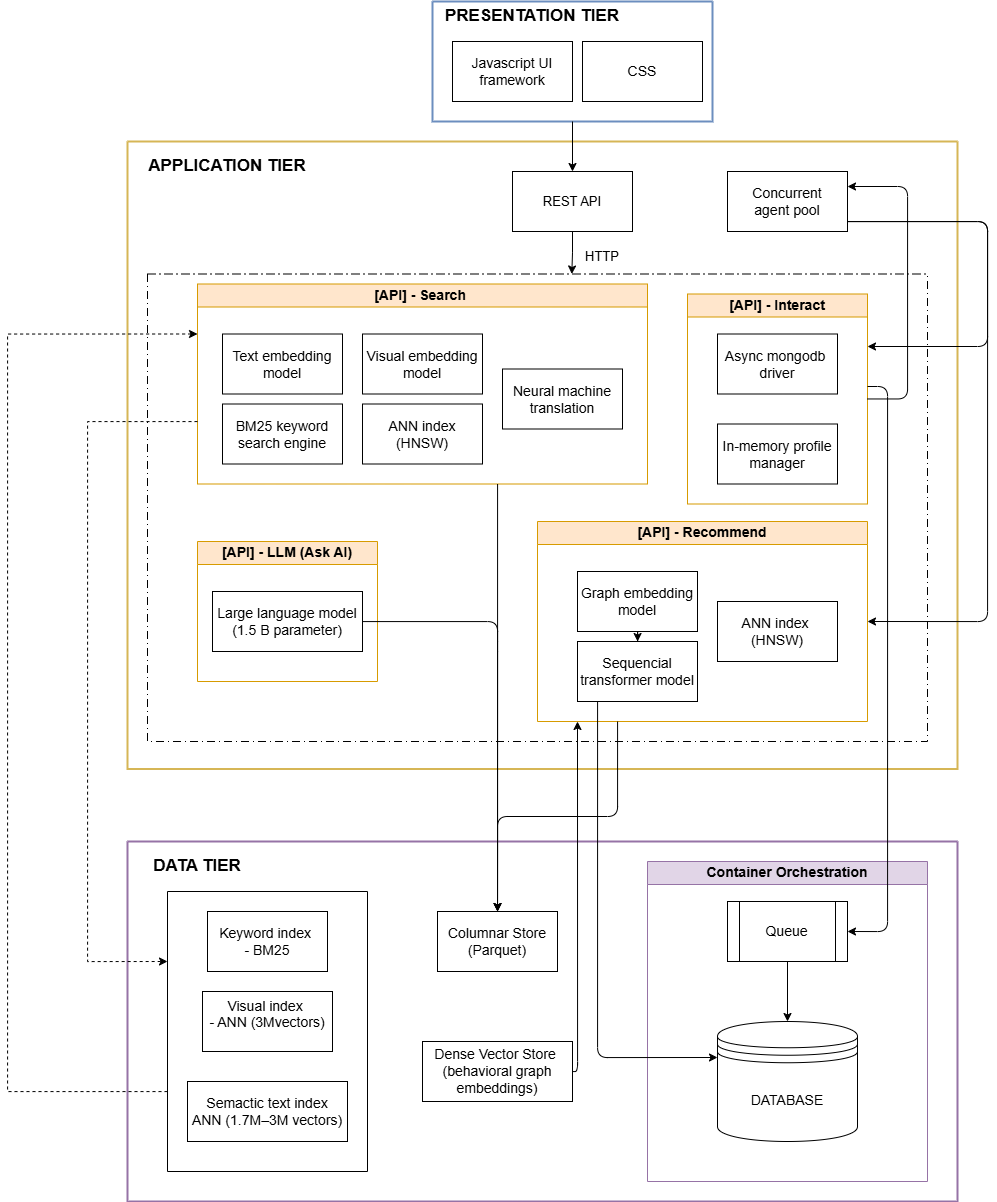
\includegraphics[width=0.90\textwidth]{Captsone/images/chapter3/Final3Tier.png}
\caption{High-level three-tier system architecture. The presentation tier communicates with the application tier exclusively through REST API calls. The data tier is accessed only by the application tier services.}
\label{fig:system_overview}
\end{figure}

\subsection{Presentation Tier}

The presentation tier is a single-page application built with React~19 and bundled by Vite.
It presents three primary views to the user: a search view that accepts free-text or image queries and displays ranked results; a recommendation view that surfaces personalised suggestions based on the user's profile; and a profile view that shows the user's interaction history and allows preference adjustments.
Communication with the backend is handled exclusively through HTTP REST calls; the frontend holds no business logic and no local data indices.

\subsection{Application Tier}

The application tier is implemented in Python~3.11 using the FastAPI framework, served by uvicorn.
It is organised into the following route modules:

\begin{itemize}
    \item /search: Accepts a text or image query, encodes it, and retrieves ranked candidates from the FAISS and Tantivy indices via Reciprocal Rank Fusion.
    \item /recommend: Returns personalised recommendations for an authenticated user by invoking the recommendation service.
    \item /interact: Records user clicks, ratings, and purchases to MongoDB and updates the in-memory user profile.
    \item /profile: Exposes the current user's embedding profile for inspection and manual override.
    \item /auth: Handles user registration, login, and JWT token issuance.
    \item /llm: Provides a conversational interface backed by a language model for query elaboration.
\end{itemize}

At startup, the application loads the FAISS index, Tantivy index, and the text encoder into memory via a lifespan context manager, so that inference infrastructure is initialised once and shared across all requests.

\subsection{Data Tier}

The data tier consists of four storage components:

\begin{itemize}
    \item MongoDB: Persists data in two collections under the \texttt{nba\_logs} database. The \texttt{interactions} collection stores raw user–item event documents (click, cart, skip) as they are drained from the Redis queue. The \texttt{profiles} collection stores the latest aggregated profile summary for each user, maintained via upsert operations.
    \item Redis: Acts as an asynchronous interaction write-queue. Every user action (click, cart, skip) is pushed onto the \texttt{nba\_interactions} list via \texttt{RPUSH}; a background worker drains the queue into MongoDB via \texttt{BLPOP} and triggers a Cleora graph refit when a configurable interaction threshold is reached.
    \item FAISS flat index: An exact inner-product search index over 3{,}080{,}829 item embeddings encoded with the BLaIR text encoder, stored as a contiguous float32 matrix on disk and loaded into CPU RAM at startup.
    \item Tantivy index: A BM25 full-text index over item titles and descriptions, built offline and served via a Python binding at query time.
\end{itemize}

Item metadata (title, author, genre, image URL) for all 3 million items is served from an \texttt{item\_metadata.parquet} file via a repository layer that reads and caches rows on demand.

